\section{bench60}\label{app:bench60}

\begin{definition}[bench60, full rule]\label{def:bench60full}
Let $g_0=3$ and $g_{10}=574{,}959$ be the least and the largest value of $g$ on MS640 at budget $10^6$, and
let $\rho=(g_{10}/g_0)^{1/10}\approx3.37$. \emph{Bin} $b\in\{0,\dots,9\}$ is the set of $P\in$ MS640 with
$g_0\rho^{b}\le g(P)<g_0\rho^{b+1}$ (bin $9$ closed on the right). \textbf{bench60} takes $6$ presentations from every
bin by the following rule.
\begin{enumerate}
  \item Over the whole subset, minimise the number of pairs of chosen presentations in the same $\Aut(\F_2)$-orbit.
  \item Subject to (1), sort the presentations of each bin by path length, the number of S-moves in the solution GS-SUB finds; break ties by smaller $g$ first, then by line number in MS640.
  Take the $6$ presentations closest to $6$ evenly spaced positions of this sorted list, the first and the last
  position included.
  % This one needs more explaination
\end{enumerate}
\end{definition}

Figure~\ref{fig:bench60} shows where the $60$ rows lie in MS640.

\begin{center}
\begin{tabular}{rrrrr}
\toprule
bin $b$ & range of $g$ & rows of MS640 & rows of bench60 & mean $g$ on bench60\\
\midrule
0 & $[3,\,11)$ & $317$ & $6$ & $6.3$\\
1 & $[11,\,35)$ & $89$ & $6$ & $17.7$\\
2 & $[35,\,116)$ & $63$ & $6$ & $74.3$\\
3 & $[116,\,390)$ & $60$ & $6$ & $261.7$\\
4 & $[390,\,1{,}314)$ & $31$ & $6$ & $691.2$\\
5 & $[1{,}314,\,4{,}433)$ & $26$ & $6$ & $1{,}746.8$\\
6 & $[4{,}433,\,14{,}959)$ & $28$ & $6$ & $9{,}869.2$\\
7 & $[14{,}959,\,50{,}482)$ & $14$ & $6$ & $19{,}596.3$\\
8 & $[50{,}482,\,170{,}367)$ & $6$ & $6$ & $66{,}530.7$\\
9 & $[170{,}367,\,574{,}959]$ & $6$ & $6$ & $353{,}647.7$\\
\midrule
all & & $640$ & $60$ & \\
\bottomrule
\end{tabular}
\end{center}

\begin{figure}[ht]
\centering
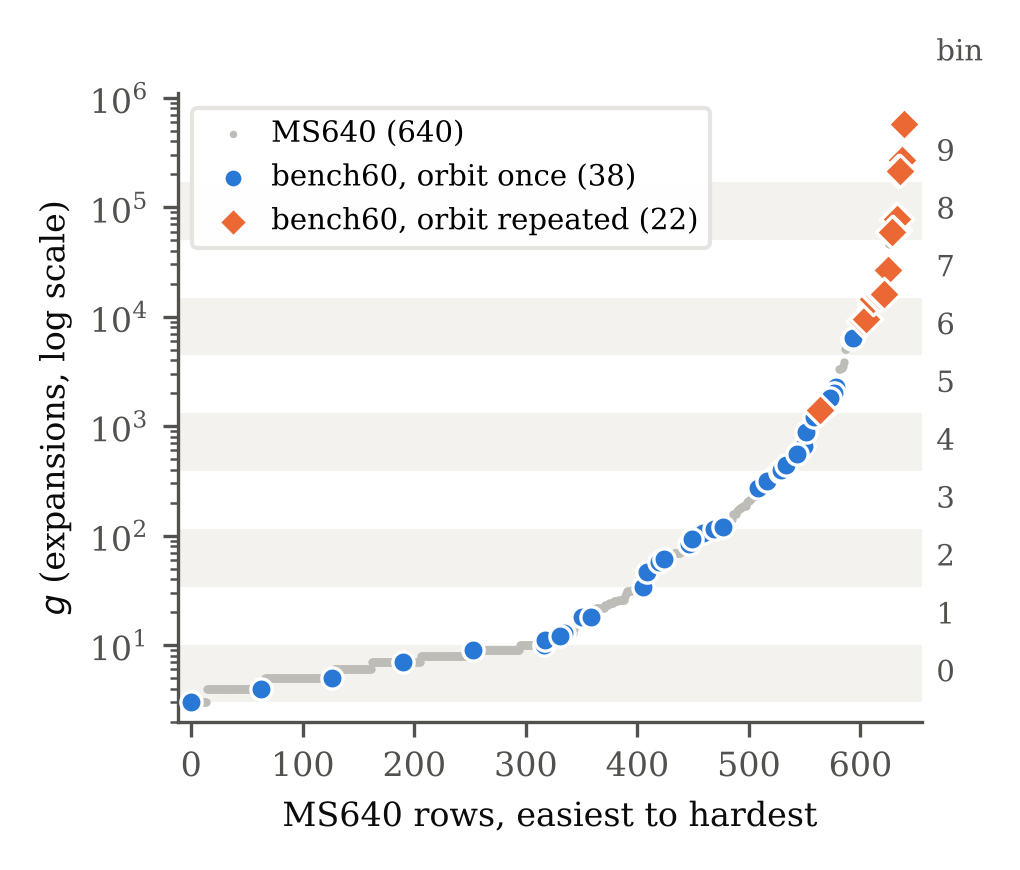
\includegraphics[width=0.49\textwidth]{figures/bench60_g.png}\hfill
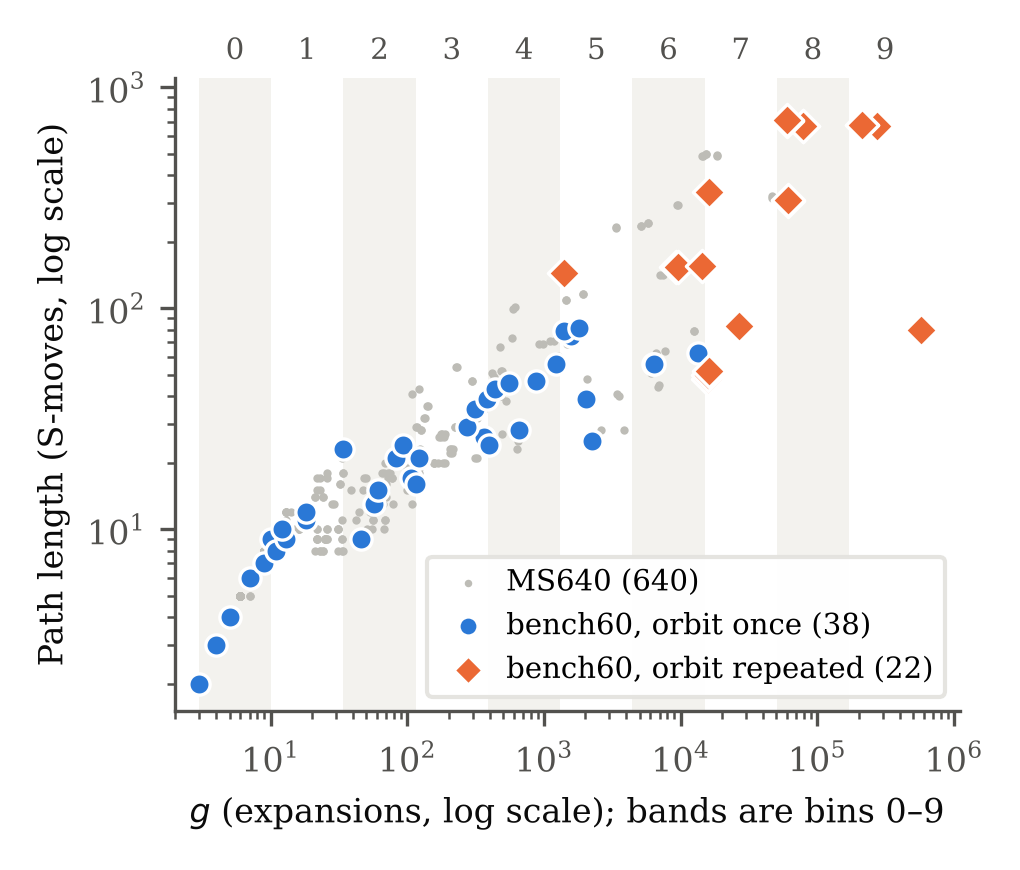
\includegraphics[width=0.49\textwidth]{figures/bench60_path.png}
\caption{bench60 inside MS640. Grey: all $640$ presentations; colour: the $60$ choices, six per bin. Blue circles are choices whose
$\Aut(\F_2)$-orbit occurs once in bench60; diamonds are choices that share an orbit with another choice, which bins 7--9 force.
Left: $g$ against the rows sorted by $g$; the shaded bands are bins 0--9, each $3.37$ times the one below.
Right: the S-move length of a presentation against $g$.}
\label{fig:bench60}
\end{figure}
